\chapter{Résoudre un Rubik's cube}

\section{Modéliser un Rubik's Cube}

Dans ce projet, nous nous sommes rendu compte que modéliser un Rubik's Cube était moins trivial qu'il n'en avait l'air.
Le modèle qu'on cherchait devait respecter plusieurs critères. 
\begin{enumerate}
    \item Premièrement nous devions avoir une interface pour récupérer la couleur de chaque facette à tout moment.
    \item Ensuite il fallait qu'on ait une fonction qui simule une rotation sur une couronne quelquonque.
    \item Enfin, notre modélisation devait être assez efficace pour permettre une résolution qui ne prenne pas trop de temps.
\end{enumerate}
\subsection{Les premières idées naïves}

\subsubsection{Le tableau de facettes}
La première idée qui nous est venue est de stocker la couleur de chaque facette dans un tableau.
Cette méthode n'est pas très efficace: créer une fonction pour simuler la rotation d'une couronne s'avère être compliqué.
De plus la complexité en mémoire n'est pas très bonne.

\subsubsection{La liste chaînée}
Similairement à cette première méthode, nous avons également songé à stocker les couleurs dans une liste chaînée en 2 dimensions.
On aurait "mis à plat" le Rubik's Cube et on aurait parcouru ses facettes sur un plan infini.

\subsubsection{Les cubies}
La deuxième idée que nous avons eu était de considérer les \textit{cubies}, petits cube constituant le Rubik's Cube en 3x3x3.
La rotation semblait être plus facile car nous aurions pu travailler avec des transformations d'angles et de position dans l'espace.
Cependant cette méthode faisait apparaître des complications d'implémentations rendant notre code très lourd.

\subsection{Le tableau de permutations}
Nous avons finalement décidé d'adopter une approche plus mathématique : le tableau de permutations.

Cela consiste en un tableau de 6*8=48 cases (six faces et 8 facettes qui peuvent bouger).
Le Rubik's résolu est alors représenté par un tableau rempli de 0 à 47 (dans l'ordre).
Effectuer une rotation est alors équivalent à appliquer une permutation sur le tableau.
Cela s'implémente simplement et l'algorithme est efficace.
Retrouver la couleur en fonction du numéro dans la case du tableau est aisé en définissant les permutations.

\begin{figure}[h]
\begin{center}
    \makebox[\textwidth]{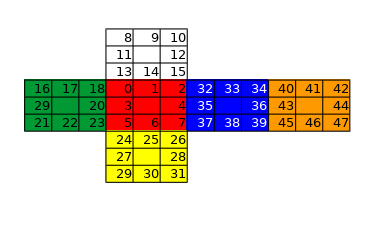
\includegraphics[width=.5\paperwidth]{diagrammes/perm.png}}
\end{center}
    \caption{Les permutations du Rubik's}
\end{figure}

C'est finalement cette approche que nous avons décidé de garder car elle nous permettait de garder un code simple et efficace.

\section{Algorithme de résolution}
Une fois que nous avons créé un objet représentant le cube que nous pouvions manipuler virtuellement, nous nous sommes attaqué à la partie résolution.
Résoudre un Rubik's Cube nécessite d'être rigoureux et surtout méthodique.
C'est donc pourquoi nous avions initialement pensé qu'un ordinateur serait parfaitement adapté pour appliquer une méthode de résolution.
Cependant, nous nous sommes aperçu que il y a toujours une partie 

